\documentclass[11pt,a4paper,twoside,openright]{report}

\usepackage[top=25mm,bottom=25mm,right=25mm,left=30mm,head=12.5mm,foot=12.5mm]{geometry}
\let\openright=\cleardoublepage

\usepackage[a-2u]{pdfx}

\usepackage[
   backend=biber
%  ,style=iso-authoryear
  ,style=alphabetic
  ,citestyle=numeric
  ,sortlocale=cs_CZ
  ,bibencoding=UTF8
  %,block=ragged
]{biblatex}
\addbibresource{references.bib}

%% Přepneme na českou sazbu, fonty Times New Roman a kódování češtiny
\usepackage[czech]{babel}
\usepackage{times}
\usepackage[T1]{fontenc}
\usepackage{textcomp}
\usepackage[utf8]{inputenc}

%%% Další užitečné balíčky (jsou součástí běžných distribucí LaTeXu)
\usepackage{amsmath}        % rozšíření pro sazbu matematiky
\usepackage{amsfonts}       % matematické fonty
\usepackage{amsthm}         % sazba vět, definic apod.
\usepackage{bm}             % tučné symboly (příkaz \bm)
\usepackage{graphicx}       % vkládání obrázků
\usepackage{fancyvrb}       % vylepšené prostředí pro strojové písmo
\usepackage{fancyhdr}       % prostředí pohodlnější nastavení hlavy a paty stránek
\usepackage{icomma}         % inteligetní čárka v matematickém módu
\usepackage{dcolumn}        % lepší zarovnání sloupců v tabulkách
\usepackage{booktabs}       % lepší vodorovné linky v tabulkách
\makeatletter
\@ifpackageloaded{xcolor}{
   \@ifpackagewith{xcolor}{usenames}{}{\PassOptionsToPackage{usenames}{xcolor}}
  }{\usepackage[usenames]{xcolor}} % barevná sazba
\makeatother
\usepackage{multicol}       % práce s více sloupci na stránce
\usepackage{caption}
\usepackage{enumitem}
\usepackage{lipsum}
\setlist[itemize]{noitemsep, topsep=0pt, partopsep=0pt}
\setlist[enumerate]{noitemsep, topsep=0pt, partopsep=0pt}
\setlist[description]{noitemsep, topsep=0pt, partopsep=0pt}
\usepackage{pdfpages}

% typografie obsahu, seznamů atp.
\usepackage{tocloft}
\setlength\cftparskip{0pt}
\setlength\cftbeforechapskip{1.5ex}
\setlength\cftfigindent{0pt}
\setlength\cfttabindent{0pt}
\setlength\cftbeforeloftitleskip{0pt}
\setlength\cftbeforelottitleskip{0pt}
\setlength\cftbeforetoctitleskip{0pt}
\renewcommand{\cftlottitlefont}{\Huge\bfseries}
\renewcommand{\cftloftitlefont}{\Huge\bfseries}
\renewcommand{\cfttoctitlefont}{\Huge\bfseries}

% vyznaceni odstavcu
\parindent=0pt
\parskip=11pt

% zakaz vdov a sirotku - jednoradkovych pocatku ci koncu odstavcu na prechodu mezi strankami
\clubpenalty=1000
\widowpenalty=1000
\displaywidowpenalty=1000

% nastaveni radkovani
\renewcommand{\baselinestretch}{1.5}

% nastavení hlavy a paty stránek
\fancyhf{}
\renewcommand{\chaptermark}[1]{\markboth{#1}{}}
\fancyhead[RO,LE]{\leftmark}
\fancyfoot[RO,LE]{\thepage}
%\renewcommand{\footrulewidth}{0pt}
\fancypagestyle{plain}{%
\fancyhf{} % clear all header and footer fields
\fancyfoot[RO,LE]{\thepage}
\renewcommand{\headrulewidth}{0pt}
%\renewcommand{\footrulewidth}{0.5pt}
}

%nastavení záhlaví a zápatí pro dvoustranný formát (lichá a sudá strana)

%pro nastavení např. pouze na pravé straně:
% \fancyhead[RO,RE]{\leftmark}
% \fancyfoot[RO,RE]{\thepage}


% Tato makra přesvědčují mírně ošklivým trikem LaTeX, aby hlavičky kapitol
% sázel příčetněji a nevynechával nad nimi spoustu místa. Směle ignorujte.
\makeatletter
\def\@makechapterhead#1{
  {\parindent \z@ \raggedright 
   \Huge\bfseries \thechapter. #1
   \par\nobreak
   \vskip 20\p@
}}
\def\@makeschapterhead#1{
  {\parindent \z@ \raggedright 
   \Huge\bfseries #1
   \par\nobreak
   \vskip 20\p@
}}
\makeatother

% Zapne černé "slimáky" na koncích řádků, které přetekly, abychom si
% jich lépe všimli.
\overfullrule=1mm

%% Balíček hyperref, kterým jdou vyrábět klikací odkazy v PDF,
%% ale hlavně ho používáme k uložení metadat do PDF (včetně obsahu).
%% Většinu nastavítek přednastaví balíček pdfx.
\hypersetup{unicode}
\hypersetup{breaklinks=true}
\hypersetup{hidelinks}

%%% Prostředí pro sazbu kódu, případně vstupu/výstupu počítačových
%%% programů. (Vyžaduje balíček fancyvrb -- fancy verbatim.)

\DefineVerbatimEnvironment{code}{Verbatim}{fontsize=\small, frame=single}



\def\NazevPrace{Grafický visuální styl gymnasia}
\def\Trida{4.B}
\def\AutorPrace{Kateřina Zusková}
\def\DatumOdevzdani{2023}

% Vedoucí práce: Jméno a příjmení s~tituly
\def\Vedouci{Šimon Schierreich}

% Studijní program a obor
\def\StudijniProgram{studijní program}
\def\StudijniObor{studijní obor}

% Text čestného prohlášení
\def\Prohlaseni{Prohlašuji, že jsem svou práci vypracoval samostatně a použil jsem pouze prameny a literaturu
uvedené v~seznamu bibliografických záznamů. Nemám žádné námitky proti zpřístupňování této práce v~souladu se
zákonem č. 121/2000 Sb. o~právu autorském, o~právech souvisejících s~právem autorským a
o~změně některých zákonů (autorský zákon) ve znění pozdějších předpisů.}

% Text poděkování
\def\Podekovani{%
Poděkování.
}

% Abstrakt česky
\def\Abstrakt{%
Práce se zabývá tvorbou visuální identity Gymnázia Jana Keplera, sestavením grafického manuálu k její aplikaci a přípravou šablon usnadňujících její použití.
}

% Abstrakt anglicky
\def\AbstraktEN{%
Abstract.
}

% 3 až 5 klíčových slov
\def\KlicovaSlova{visuální identita, grafický manuál, šablona}
% 3 až 5 klíčových slov anglicky
\def\KlicovaSlovaEN{keyword, important term, another topic, and another one}


\begin{document}

%%% Titulní strana práce a další povinné informační strany

%%% Titulní strana práce

\pagestyle{empty}
\pagenumbering{gobble}
\hypersetup{pageanchor=false}

\begin{center}
\LARGE
\textbf{GYMNÁZIUM JANA KEPLERA}\\
{\large Parléřova 2/118, 169 00 Praha 6}

\vspace{\stretch{3}}


\includegraphics[width=.4\textwidth]{img/logo}

\vspace{\stretch{3}}

{\Huge\bfseries\NazevPrace}

\vspace{8mm} 
Maturitní práce

\vspace{\stretch{8}}
\large
\begin{tabular}{rl}
Autor: & \AutorPrace \\
\noalign{\vspace{2mm}}
Třída: & \Trida\\
\noalign{\vspace{2mm}}
Školní rok: & \SkolniRok\\
\noalign{\vspace{2mm}}
Předmět: & \Predmet \\
\noalign{\vspace{2mm}}
Vedoucí práce: & \Vedouci \\
\end{tabular}

\vspace{20mm}
Praha, \DatumOdevzdani
\end{center}


\openright


% zadani viz šablona zadání


\includepdf[]{sablona_zadani.pdf}

%%% Poděkování
\openright
\vspace*{\fill}
\section*{Poděkování}
\noindent
\Podekovani
\vspace{1cm}


%%% Strana s čestným prohlášením k bakalářské práci

\hypersetup{pageanchor=true}
\cleardoublepage
\vspace*{\fill}
\section*{Prohlášení}
\noindent
\Prohlaseni

\vspace{2cm}
\noindent
V Praze dne \today
\hspace*{\fill}\small{\AutorPrace}
\vspace{1cm}


%%% Povinná informační strana bakalářské práce
\openright
\section*{Abstrakt}
\noindent
\Abstrakt
\subsection*{Klíčová slova}
\noindent
\KlicovaSlova

\vfill

\section*{Abstract}
\noindent
\AbstraktEN
\subsection*{Keywords}
\noindent
\KlicovaSlovaEN

\openright
\pagenumbering{arabic}

% Obsah
\setcounter{tocdepth}{2}
\tableofcontents

\chapter{Teoretická část}
\pagestyle{fancy}

% V první části maturitní práce by se měla objevit informace o tom, jaký problém řešíte. Co si Váš projekt klade za cíl?


% CÍL

Cílem práce je sjednotit vizuální styl Gymnázia Jana Keplera, sestavit grafický manuál udávající pravidla tohoto stylu, vytvořit základní šablony pro usnadnění jeho používání (vizitky, dopisní papír, prezentace, závěrečné práce, emailový podpis) a navrhnout úpravy webových stránek školy.
Cílem není vytvořit vizuální identitu novou.

% Gymnázium Jana Keplera nemá sestavený žádný grafický manuál. Jeho visuální identita je nejasná a používána nejednotně a bez pravidel. Mým cílem je sestavit grafický manuál, který by měl zabránit nejednotě visuální komunikace, definovat a zpřehlednit jeho visuální identitu tak, aby s ní bylo možné snadno pracovat. Grafický manuál by měl určovat, jak používat logo, barvy, fonty a další grafické prvky. Zároveň je sestaven tak, aby se jím mohl řídit jakýkoliv designér používající jakékoliv médium.
% Dále je mým cílem sestavit šablony usnadňující použití visuální identity v nejpoužívanějších médiích pro často užívané dokumenty a další náležitosti a navrhnout úpravy webových stránek tak, aby byly v souladu s grafickým manuálem.

% **logoxlogotypxpiktogram**
% **v implementaci mám možná info hodící se spíše do teoretické sekce - VYŘEŠIT**

\section{Analýza značky}
Prvním krokem k tvorbě dobrého designu je analýza značky. Cílem této fáze je ujasnit, jaké jsou hlavní myšlenky a hodnoty značky, její účel, čím se odlišuje a jak chce vystupovat na veřejnosti. Další nezbytnou součástí je analýza cílové skupiny a konkurence. Na základě této analýzy se sestavuje verbální, vizuální a emoční identita značky, tj. jak by značka měla působit. Sice není cílem vizuální styl školy zcela změnit a ráda bych se držela již stávajících prvků, i tak je však analýza potřebná pro vytvoření co nejlepších designů.

Analýza značky byla provedena na základě konzultace se zástupkyní ředitele Mgr. Marcelou Grabmüllerovou a na základě informací poskytnutých na webu školy. Analýza konkurence byla provedena převážně na základě webových stránek konkurenčních škol a některých dokumentů poskytovaných online, zanalyzována byla tedy především její vizuální identita.

Výsledky analýzy značky jsou následující:

\textbf{Cíli značky}  jsou výchova a komplexní vzdělávání nadaných studentů a jejich příprava na VŠ.
\textbf{Cílem propagace} je získat nadané studenty a kvalitní pedagogy.
\textbf{Cílovou skupinou} jsou hlavně rodiče, ale také potenciální kvalitní studenti a pedagogové. Škola cílí převážně na skupiny, které vyhledávají kvalitu, otevřenost, spolehlivost a příležitosti. Vzhledem k tomu, že se jedná o českou školu, cílí především na západoevropskou kulturu.
\textbf{Hodnotami značky} jsou prestiž, úspěch, kvalita, individualita a otevřenost. \textbf{Odlišuje se} právě individualitou, které dosahuje například širokou škálou volitelných seminářů.
\textbf{Verbální identita} značky je přátelská, ale zároveň seriózní.
\textbf{Emoční identita} značky se skládá z následujícího: značka by měla působit moderně, vzbuzovat dojem kvality a úspěchu, svobody, přátelskosti a podpory. Těchto hodnot škola dosahuje například moderním vybavením, bezbariérovým přístupem, dostupností školního psychologa a širokou nabídkou studijních příležitostí.\cite{svp}

Výsledky analýzy konkurence jsou následující:

\textbf{PORG} užívá hlavně modrou a bílou barvu, kombinuje patkové a bezpatkové písmo. Web působí moderně, jeho obsah je přes celou plochu obrazovky. Obsahuje mnoho fotografií a videí. Působí kvalitně a osobně.\cite{porg}

\textbf{Gymnázium Nad Alejí} má webové stránky převážně bílé s modrými a oranžovými nápisy. V logu užívá také zelenou barvu. Používá převážně bezpatkové písmo, použítí písem je ale nejednotné. Web působí nedodělaně, nepřehledně a zastarale.\cite{alej}\cite{einstein}

\textbf{Gymnázium Na Zatlance}

Kromě analýzy konkurence jsem také zanalyzovala vizuální identitu některých zahraničních gymnázií:
% dát to sem? neznám autory webu :(((

\section{Grafický manuál}
Grafický manuál by měl zabránit nejednotě vizuální komunikace, definovat a zpřehlednit jeho vizuální identitu tak, aby s ní bylo možné snadno pracovat. Měl by určovat, jak používat logo, barvy, fonty a další grafické prvky související se značkou. Zároveň by měl být sestaven tak, aby se jím mohl řídit jakýkoliv designér používající jakékoliv médium.

\subsection{Logo}
Kvůli licenci fontu bylo potřebné změnit font textu okolo loga.
Rozhodla jsem se také navrhnout variantu loga, kdy je logo použito s textem orientovaným horizontálně v bloku vedle portrétu - na webových stránkách je momentálně logo (portrét s textem v kruhu) i s horizontálně orientovaným textem, tudíž se text dvakrát opakuje (viz \nameref{fig:logo_web}). V nově vytvořeném logu s horizontálním textem je také místo nápisu "Gymnasium Jana Keplera" použit nápis "Gymnázium Jana Keplera." Působí to moderněji a přirozeněji.

Vytvořila jsem také obě varianty loga v invertovaných barvách. Tyto varianty však nemají pouze prohozené barvy, invertovaný portrét je tvořen obrysem. Kdyby byly pouze invertované barvy, portrét by "zapadl dovnitř" a z estetického hlediska by nebyl dobrý.

Nezbytnou součástí grafického manuálu jsou také nepovolené varianty loga. Těmi jsou například čistě invertované logo bez použití obrysu nebo logo s dvojím textem okolo portrétu a horizontálně v bloku vedle něj.

\begin{figure}[htbp]
  
\includegraphics[width=1\textwidth]{img/gjk_web_hlavicka.png}
  \caption{logo na webu www.gjk.cz}
  \label{fig:logo_web}
\end{figure}

%
\includegraphics[width=1\textwidth]{img/gjk_web_hlavicka.png}
%    \caption{logotyp na webu gjk}
%    \label{fig:logotyp_web}

V nově vytvořeném logu s textem zakřiveném do kruhu v novém fontu bylo nutné prostrkat písmena tak, aby byl vizuálně vyvážený. Postup jsem konzultovala s Janem Čumlivskim na UMPRUM.

Důležitá je také tvorba ochranné zóny - prázdného prostoru kolem loga, který zajišťuje, že logo bude čitelné a nebude se při použití překrývat s jinými objekty. Vytvořena byla následovně: vybrala jsem část loga a její velikost jsem označila jako x. Po všech stranách loga jsem vytvořila prázdný prostor např. o velikosti 2x. Přesnější specifikace ochranné zóny u jednotlivých log je uvedena v grafickém manuálu.

\subsection{Barvy}
Vzhledem k tomu, že škola zjevně používá odstíny modré jako primární barvu, rozhodla jsem se modré barvy držet a pouze pozměnit odstíny tak, aby lépe ladily a aby vypadaly dobře jak na tiskovinách, tak na digitálních zařízeních.

Modrá barva má dokonce své opodstatnění i podle psychologie barev. Modrá barva zklidňuje. Použití modré nebo jiných studených barev je vhodné, chceme-li propagovat něco, co vyžaduje pečlivé zhodnocení a delší rozhodování (narozdíl např. od oranžové, která podporuje spontánní rozhodování). Těchto poznatků se hojně využívá v obchodních centrech, v interier designu, ale také v medicíně.
\cite{enwiki:1144176285}
Často je asociována s bezpečím, spolehlivostí, důvěrou a kvalitou.\cite{hallock}
Modrá barva je v západní kultuře často spojována s úspěchem a s jistotou, což se také hodí pro potřeby školy. \cite{grafika}

Dalším důležitým poznatkem je, že lidé obecně preferují, pokud jsou barvy různých prvků v podobných odstínech, nejedná-li se např. o text a pozadí, kde je naopak vyžádován kontrast.\cite{enwiki:1144176285}\cite{color} Tento kontrast ovšem nesmí být příliš velký, mohl by potom způsobovat tzv. vibrace, které můžou působit agresivně a zvýšit obtížnost čtení.\cite{grafika}
%https://www.onlio.com/-/psychologie-barev-dokonceni
%kniha
% https://www.youtube.com/watch?v=XNkV6m4fosw

\subsection{Písmo}
\label{sec:písmo}
Jako písmo na logo bylo nutné zvolit font s otevřenou licencí podporující celou českou abecedu. Chtěla jsem, aby působil moderně, snadno se četl, ale zároveň nebyl zcela obyčejný. Pro tyto účely jsem zvolila druh písma \footnote{https://fonts.google.com/specimen/Prompt}. Rozhodla jsem se jej určit i jako primární písmo pro nadpisy.
Jako písmo pro delší texty (obsah sdělení) jsem se rozhodla na základě konzultace na UMPRUM použít font Arial Regular. Tento font se dobře čte, většina lidí je na něj zvyklá a používá se na webových stránkách školy, tudíž to nebude pro čtenáře taková změna.
Pro delší dokumenty (závěrečné práce atp.) jsem zvolila patkové písmo Times New Roman pro jeho dobrou čitelnost - patkové písmo se hodí pro rozsáhlé texty\cite{grafika} a právě písmo Times New Roman je i podle studií považováno za jedno z nejlépe čitelných.\cite{times} Kompilátor pdfLaTeX navíc umí pracovat pouze s Times New Roman.

\section{Šablony}
\subsection{Nejčastěji používaný software}
Vzhledem k tomu, že šablony dělám primárně pro vedení školy a pro studenty, jsem se rozhodla udělat průzkum o nejčastěji používaném softwaru (viz \nameref{part:prilohy} - příloha 1). Na základě konzultace s Mgr. Marcelou Grabmüllerovou jsem zjistila, že veškeré šablony pro vedení školy by měly být, pokud možno, dostupné hlavně pro Google platformu. Nejčastěji používaný software mezi studenty jsem zjišťovala pomocí rozeslaného dotazníku.
% dotazník je dostupný zde a zde
% výsledky dotazníku

Šablony budu tedy tvořit primárně pro Google platformu a Microsoft Office (šablony z Google platformy lze konvertovat přímo pro Microsoft Office), šablony maturitní práce pak také v LaTeXu. Výjimkou jsou šablony vizitek a emailového podpisu, pro které tento software není vhodný.

\subsection{Závěrečná práce a zadání závěrečné práce}
Funkcí šablony je sjednotit styl závěrečných prací. Vzhledem k rozmanitosti předmětů, v rámci kterých závěrečné práce vznikají, nemohou mít všechny závěrečné práce stejnou strukturu a totožný vzhled. Účelem je tedy sjednotit základní prvky jako font, velikost písma, pořadí některých prvků (poděkování, abstrakt, prohlášení..) a podobně. Součástí šablony závěrečné práce je titulní strana, která by, podobně jako šablona zadání, měla být pro všechny předměty totožná.
Na šabloně zadání závěrečné práce bude pravděpodobně pracovat jak student, tak vedoucí práce, v některých případech pouze vedoucí práce.

Podoba závěrečné práce je inspirována původní šablonou, jelikož nevidím důvod výrazně měnit vzhled maturitních prací. Inspirovala jsem se také vzhledem bakalářských prací FIT ČVUT. \footnote{https://dspace.cvut.cz/handle/10467/3577} Rozhodla jsem se však pro černobílé provedení, jelikož většina studentů své práce tiskne na vlastní náklady a černobílý tisk je ve většině případů levnější než tisk barevný.

Šablonu závěrečné práce jsem se rozhodla vytvořit na základě požadavků pro maturitní práci z humanitních studií. Podmínky povolují fonty Arial, Georgia a Times New Roman (více o důvodech zvolení písma Times New Roman viz \nameref{sec:písmo}).

\subsection{Dopisní papír}
\subsection{Email}
\subsection{Prezentace}
https://mirrors.nic.cz/tex-archive/macros/latex/contrib/beamer/doc/beameruserguide.pdf
\subsection{vizitky}
https://www.verso.cz/Upload/Priprava-dat-pro-vizitky.pdf
https://startujemeweby.cz/blog/standardni-rozmery-vizitek-jak-vybrat-ty-spravne/
nezapomenout na spadávku (asi ne google docs, ale inkscape)

inspiraci jsem čerpala z vizitek ČVUT a UK, ale také Oxfordu, Cambridge atp. Některé návrhy jsou také z mé hlavy.
https://www.forbes.com/advisor/business/best-business-card-designs/
https://venngage.com/blog/business-card-examples/

http://papirovydrak.cz/jak-pripravit-data-pro-tisk/
https://www.topvizitky.cz/jak-pripravit-podklady/

vizitka není velký nápis jména atp... protože...
\section{Návrhy úprav webových stránek}



\chapter{Implementace}

Druhá kapitola obsahuje detailní informace o tom, jak probíhala implementace. Zde se objeví zdůvodnění výběru technologií, řešení problémů, na které jste narazili, informace o použitých knihovnách apod. Pochvalte se, nikdo to za Vás neudělá. Přiznejte chyby, není to ostuda.

\section{Vektorová grafika}
\label{sec:grafika}
Nedílnou součástí projektu je tvorba grafiky. Ačkoli škola například logo má a mým úkolem není vymýšlet logo nové, je potřeba ho zvektorizovat a navrhnout povolené a zakázané varianty. 

Pro loga, logotypy atp. je nejlepší vektorová grafika, aby bylo možné různě upravovat jejich velikost a podobu bez ztrát na kvalitě.

Pro tvorbu vektorové grafiky se v profesionálním prostředí nejčastěji používá software od Adobe nebo Affinity. Tyto možnosti jsem však zavrhla (viz \nameref{sec:manual}).

Nejznámějšími programy pro tvorbu grafiky zdarma jsou Inkscape, GIMP a Krita. Existuje samozřejmě mnoho dalších, většina mě známých však nemá dostatek nástrojů nebo je ve vývoji.
GIMP je podle definice "multiplatformní nástroj pro manipulaci s fotografiemi“ a používá rastrovou a bitmapovou grafiku. Na tvorbu loga atp. se tedy příliš nehodí.
Inkscape je podle definice „otevřený nástroj pro kreslení pro vytváření a úpravy grafiky SVG,“ používá vektorovou grafiku a jedná se snad o nejlepší alternativu k Adobe Illustrator, proto jsem jej zvolila jako vhodný program.
Krita také umí pracovat s vektrovou grafikou a vytvořit v ní logo je možné. Primárně ale pracuje s rastrovou grafikou a je určená hlavně pro umělce zabývající se concept artem, ilustracemi a komiksy. Inkscape je tedy vhodnější už proto, že se zabývá výhradně vektorovou grafikou a nabízí více možností z hlediska vektorové grafiky. S Inkscapem navíc mám trochu zkušeností a pracovat s Kritou, která je komplexnější, ale zároveň mnohem složitější a uživatelsky méně intuitivní, by pro mě bylo zbytečně mnohem složitější.


https://cisatrochu zkušeností a pracovat s Kritou, která je mnohem design.cz/logo-vs-logotyp/
https://daviesložitějsmediadesign.com/cs/inkscape-vs-gimp-which-one-should-you-use/
https://www.quora.com/How-would-you-compare-Inkscape-vs-Krita-Which-one-is-better-for-website-and-brand-design-including-logos

\section{Grafický manuál}
Rozhodla jsem se udělat grafický manuál v pdf. Nabízí se udělat také responzivní grafický manuál v podobě webové stránky. Webová stránka nabízí responzivitu. Nicméně forma pdf je běžnější, pro spoustu lidí srozumitelnější a vhodnější pro potřeby gymnázia. Zároveň ji lze také snadno vytisknout a používat i offline. Vzhledem k tomu, že gymnasium nepotřebuje žádný velký a detailně propracovaný grafický manuál, rozhodla jsem se jej udělat jednoduchý a forma webové stránky by jej zbytečně zesložiťovala. Zároveň by to byla spousta práce navíc, která by téměř neměla smysl.

\label{sec:manual}
K tvorbě grafického manuálu jsem se rozhodla použít sázecí program Scribus. Jedná se o open-source software, který je zdarma. Má grafické rozhraní, díky čemuž bude moct grafický manuál v budoucnosti aktualizovat i člověk, který nemá příliš zkušeností s prací se sázecími programy.

Jako další možnosti jsem zvažovala použití softwaru od Adobe nebo Affinity. Tento software je používán pro tvorbu grafických manuálů v profesionálním prostředí a určitě by nebyl špatnou volbou co se týče nabízených nástrojů. Rodina Adobe i Affinity navíc nabízí i špičkové programy pro tvorbu vektorové grafiky (více o výběru sw pro tvorbu grafiky v sekci \nameref{sec:grafika}). Bohužel, Adobe i Affinity jsou licencované produkty vyžadující nemalou investici peněz. Nabízí sice zlevněné edukační a studentské licence, ale ani tak se nejedná o zrovna levné programy. Škola by musela platit licenci, aby manuál mohl být dále aktualizován. Ačkoliv je nabízený software profesionální, nabízí spoustu možností, které nejsou pro mé potřeby nutné. Zároveň by se kdokoliv, kdo by manuál dále aktualizoval, musel se softwarem seznámit, což je pro mnohé lidi, kteří se v grafice nepohybují, u složitých programů složité. Narozdíl od Adobe a Affinity byl program Scribus využíván studenty pro sazbu školního časopisu, program je nainstalovaný na školních počítačích a obecně má na škole větší zázemí. Nástroje Scribusu bohatě stačí pro můj projekt a zároveň je zdarma. Vzhledem k tomu, že Scribus dostačuje pro mé potřeby, jsem se rozhodla do Adobe nebo Affinity neinvestovat.

Jako další možnost se jeví použítí LaTeXu. Ten je vhodný ale spíše pro práci s textem, ne s velkým množstvím grafického obsahu, který je nedílnou součástí grafického manuálu. Další nevýhodou by bylo, že budoucí aktualizace manuálu by mohli dělat pouze lidé, kteří latexu rozumí, kterých na škole není příliš velké množství. Se Scribusem sice také většina lidí běžně nepracuje, nicméně je mnohem intuitivnější.

Dále by bylo možné grafický manuál sázet v online nástrojích jako Canva, nebo dokonce i v PowerPointu. Tyto možnosti jsem ale zavhrla vzhledem k jejich omezeným možnostem a také proto, že jejich použití nepůsobí profesionálně - ačkoliv nejsem profesionál, chci, aby výsledek měl alespoň nějakou úroveň. Navíc oba programy jsou určeny pro jiné účely, tedy i proto nenabízejí tak dobré možnosti, jako Scribus, Adobe a Affinity.

Další možností je MS Publisher - je sice více uživatelsky přátelský, nemám na něj ale licenci, nenabízí tolik nástrojů, nepodporuje grafiku ve formátu svg a je dostupný pouze pro operační systémy Windows. 

Před samotnou tvorbou finální verze grafického manuálu jsem vytvářela provizorní grafický manuál v Google Sheets, jelikož v průběhu tvorby šablon jsem musela několikrát jednotlivé prvky upravovat a bylo pro mě jednodušší a rychlejší je upravovat v této aplikaci. Manuál jsem nasázela ve Scribusu až tehdy, když jsem měla finální verzi.

\subsection{logo}
Pro tvorbu loga jsem zvolila program Inkscape. V něm jsem původní logo zvektorizovala. Změnila jsem písmo na font Prompt extrabold nainstalovaný z googlefonts. Tento font má otevřenou licenci OFL, tudíž jej škola může využívat i pro propagační účely.

Další důležitou součástí tvorby loga je vytvoření ochranné zóny. Vybrala jsem velikost části logotypu a tuto velikost v jejím násobku převedla na kraj v podobě čtverce. Poté jsem změnila velikost stránky na velikost výběru.

\subsection{Barvy}
Pro práci s barevnou paletou jsem používala online nástroj Paletton\footnote{https://paletton.com/}.

\subsection{Písmo}
Druh písma Prompt jsem nalezla a nainstalovala z databáze fontů Google Fonts\footnote{https://fonts.google.com/specimen/Prompt}.

Jako písmo pro delší texty jsem zvolila písmo Arial. Vzhledem k tomu, že většina pedagogického sboru pracuje s operačním systémem Windows, je tento font vhodný i proto, že je dostupný na většině počítačů (s operačním systémem Windows) a v nejčastěji používaném softwaru, pro který navrhuji šablony (Google platforma a Microsoft Office). Font sice není v základu poskytován unixovými operačními systémy, nicméně lze doinstalovat a lidé používající tyto operační systémy jsou většinou dostatečně technicky zdatní a dokáží si font opatřit.

Jako font pro závěrečné práce a jiné delší dokumenty jsem zvolila písmo Times New Roman, protože je, narozdíl od písma Arial, podporované kompilátorem pdfLaTeX a jeho použití by tak mělo být pro uživatele snazší (např. platforma Overleaf\footnote{https://www.overleaf.com/} kompiluje primárně přes pdfLaTeX, uživatel samozřejmě může zvolit jiný kompilátor, ale práce se šablonou by kvůli tomu byla složitější). Tento font je zároveň v základu dostupný na Google platformě i v Microsoft Office. Díky tomu uživatel nemusí doinstalovávat font na žádné z platforem, pro které jsou šablony dostupné.

\section{Šablony}
\subsection{vizitky}
Pro tvorbu šablon vizitek jsem zvolila program Inkscape. Vzhledem k tomu, že jsem v něm vytvářela loga, jsem ho už zvládala na základní úrovni ovládat. Umožňuje přesnou práci a ukládat barvy ve formátu CMYK, který je pro tisk vhodnější než formát RGB. Umožňuje grafiku ukládat v křivkách, což je mnohými tiskárnami vyžadováno.

% ZKŘIVKOVAT PÍSMA, ZKONTROLOVAT DPI

% https://www.verso.cz/Upload/Priprava-dat-pro-vizitky.pdf
\subsection{Dopisní papír}
problém s bezokrajovým tiskem a doporučení na případné použití původních návrhů v případě pořízení bezokrajové tiskárny

\subsection{Maturitní práce a zadání maturitní práce}
Šablony jsem se rozhodla vytvořit úpravou již existujících LaTeXových šablon na maturitní práci z informatiky. Upravila jsem její vzhled (titulní stranu, font atd.), bibliografii, strukturu a některá makra. Tento postup jsem zvolila proto, abych nezapomněla do šablony zakomponovat důležitá makra (např. matematické balíčky, se kterými nemám zkušenosti). Zvolený postup také značně urychlil moji práci. Šablony nejsou totožné, vyskytují se v nich však podobnosti právě z tohoto důvodu.

Na šabloně zadání závěrečné práce bude pravděpodobně pracovat jak student, tak vedoucí práce, v některých případech pouze vedoucí práce. Z tohoto důvodu jsem se rozhodla šablonu zadání vytvořit jako samostatnou šablonu. Šablona zadání není součástí šablony maturitní práce pro případ, že se vedoucí prací rozhodne neposkytnout studentům přístup k šablonám, aby je nemohli upravovat a zadání zůstalo neměnné.

\section{Návhry úprav webových stránek}


\chapter{Technická dokumentace}

Poslední kapitola obsahuje informace o tom, jak projekt, který v rámci maturitní práce vznikl, nainstalovat, spustit a používat.

% PÍSMO - POZOR NA LICENCOVÁNÍ ARIAL - POUZE KDYŽ JE ZAKOUPENO (WINDOWS)
% návod jak stáhnout písmo

\section{Šablony}
\subsection{Závěrečná práce}
Šablona maturitní práce je pouze pomůckou, která má pomoci udržet podobný vizuální styl závěrečných prací a navést je k určité struktuře. Každý student by si měl ověřit, zda jeho závěrečná práce splňuje všechny podmínky (každý předmět může mít podmínky nastavené jinak). Také by měl zkontrolovat, že všechny jeho citace jsou v požadované normě. V případě LaTeXové šablony je nastavená norma ISO 160, i tak ale doporučuji překontrolování všech citací. V případě google dokumentů student musí citace generovat sám.

\section{Ukázka sekce}

\lipsum[5]

\subsection{A jedné podsekce}

\lipsum

\section{A další sekce}

\lipsum

\chapter*{Závěr}
\pagestyle{empty}
\addcontentsline{toc}{chapter}{Závěr}

Závěr obsahuje shrnutí práce a vyjadřuje se k míře splnění jejího zadání. Dále by se zde mělo objevit sebehodnocení studenta a informace o tom, co nového se naučil a jak vnímal svou práci na projektu.

%%% Seznam použité literatury
\nocite{einstein}\nocite{latexcompanion}\nocite{knuthwebsite}
\printbibliography[title={Seznam použité literatury},heading={bibintoc}]

%%% Seznam obrázků
\openright
\listoffigures
\addcontentsline{toc}{chapter}{Seznam obrázků}

%%% Seznam tabulek
\clearpage
\listoftables
\addcontentsline{toc}{chapter}{Seznam tabulek}

%%% Přílohy k práci, existují-li. Každá příloha musí být alespoň jednou
%%% odkazována z vlastního textu práce. Přílohy se číslují.

\part*{Přílohy}\label{part:prilohy}
\Large\textbf{příloha 1}
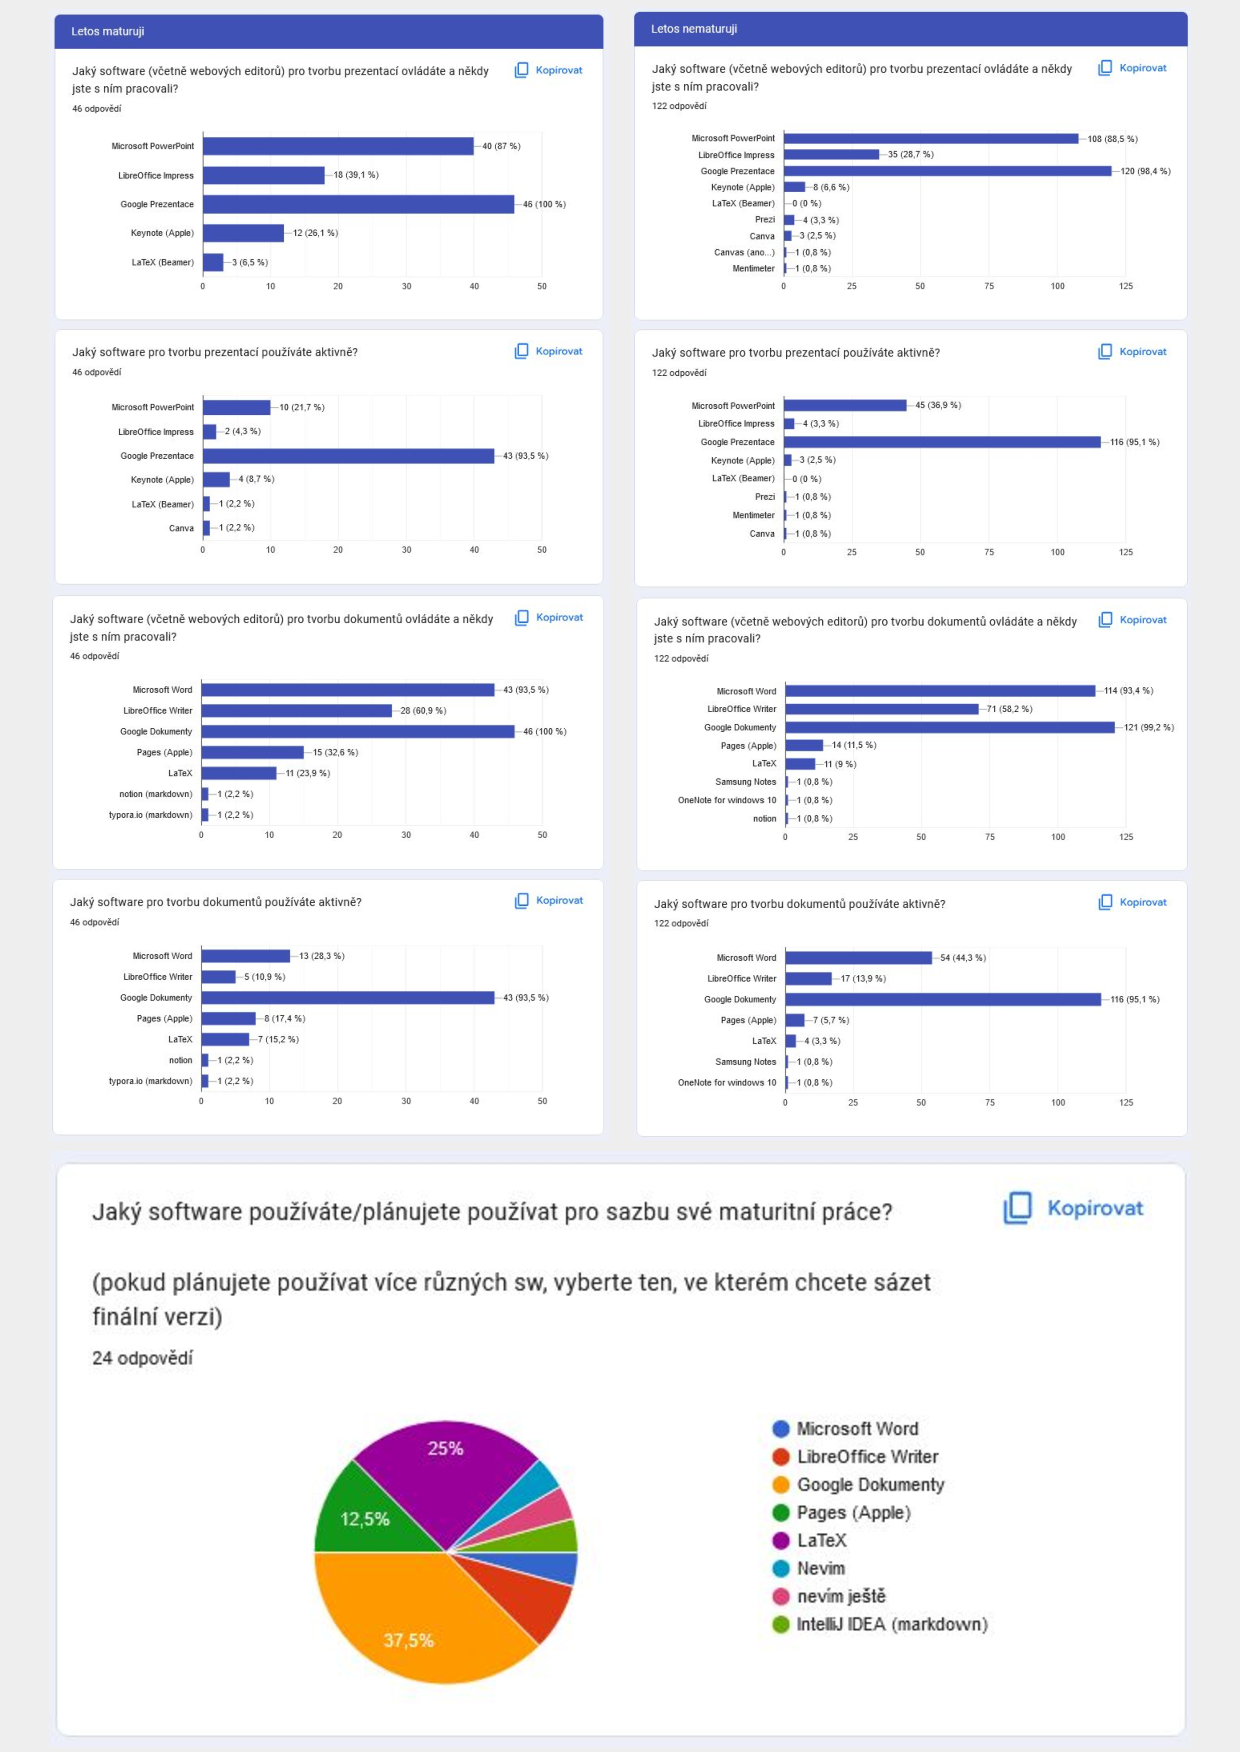
\includepdf[]{dotaznik.pdf}
% \appendix

\end{document}
